%%%%%%%%%%%%%%%%%%%%%%%%%%%%%%%%%%%%%%%%%%%%%%%%%%%%%%%%%%%%%%%%%%%%%%%%%%%%%%%%
%2345678901234567890123456789012345678901234567890123456789012345678901234567890
%        1         2         3         4         5         6         7         8

\documentclass[letterpaper, 10 pt, conference]{ieeeconf}  % Comment this line out if you need a4paper
\usepackage{amstext}
\usepackage{amsfonts}
\usepackage{float}
\usepackage{graphicx}
%\documentclass[a4paper, 10pt, conference]{ieeeconf}      % Use this line for a4 paper

\IEEEoverridecommandlockouts                              % This command is only needed if
                                                          % you want to use the \thanks command

\overrideIEEEmargins                                      % Needed to meet printer requirements.

%In case you encounter the following error:
%Error 1010 The PDF file may be corrupt (unable to open PDF file) OR
%Error 1000 An error occurred while parsing a contents stream. Unable to analyze the PDF file.
%This is a known problem with pdfLaTeX conversion filter. The file cannot be opened with acrobat reader
%Please use one of the alternatives below to circumvent this error by uncommenting one or the other
%\pdfobjcompresslevel=0
%\pdfminorversion=4

% See the \addtolength command later in the file to balance the column lengths
% on the last page of the document

% The following packages can be found on http:\\www.ctan.org
%\usepackage{graphics} % for pdf, bitmapped graphics files
%\usepackage{epsfig} % for postscript graphics files
%\usepackage{mathptmx} % assumes new font selection scheme installed
%\usepackage{times} % assumes new font selection scheme installed
%\usepackage{amsmath} % assumes amsmath package installed
%\usepackage{amssymb}  % assumes amsmath package installed

\title{\LARGE \bf
Homework 1 Report
}


\author{Arrian Chi% <-this % stops a space
}


\begin{document}



\maketitle
\thispagestyle{empty}
\pagestyle{empty}


%%%%%%%%%%%%%%%%%%%%%%%%%%%%%%%%%%%%%%%%%%%%%%%%%%%%%%%%%%%%%%%%%%%%%%%%%%%%%%%%
\begin{abstract}

In this homework, I have simulated 3 different systems: a system of 3 metal spheres connected by beams falling in a viscous liquid, the same system but with N spheres, and a bending elastic beam subject to a single point load. The findings in each of these systems is discussed in the following sections.

\end{abstract}


%%%%%%%%%%%%%%%%%%%%%%%%%%%%%%%%%%%%%%%%%%%%%%%%%%%%%%%%%%%%%%%%%%%%%%%%%%%%%%%%
\section{4.1 Rigid Spheres and Elastic Beam Falling in Viscous Flow}

In this problem, we consider 3 falling metal spheres on an elastic beam that is falling under gravity. The constants are shown in the following table:

\begin{table}[h]
\caption{Variables Involved in the System of 3 Metal Spheres}
\label{table_variables}
\begin{center}
\begin{tabular}{|c|c|c|}
\hline
Variable & Description & Sample Value \\
\hline
& & \\ $\mu$ & Viscosity of the fluid & 1000 Pa-s \\
& & \\ $\rho_{ \text{fluid} }$ & Density of the fluid & 1000 kg/m\(^3\) \\
& & \\ $\rho_{\text{metal}}$ & Density of the spheres & 7000 kg/m\(^3\) \\
& & \\ $R_1, R_2, R_3$ & Radius of each sphere & 0.005 m, 0.025 m, \\ & & 0.005 m \\
& & \\ $l$ & Length of the beam & 0.10 m \\
& & \\ $r_0$ & Cross-sectional radius  & 0.001 m \\ & of the beam & \\
& & \\ $E$ & Young's modulus & $1.0 \times * 10^{9}$ Pa \\ & of the beam & \\
& & \\ $EA$ & Stretching stiffness & $E\pi r_0^2$  \\ & of the beam & \\
& & \\ $EI$ & Bending stiffness & $E\pi r_0^4 / 4$  \\ & of the beam & \\
& & \\ $\Delta l$ & Half-length of & 0.05 m \\ & the beam & \\

& & \\ $x_1, x_2, x_3$ & x position of each & initial at 0, $\Delta l$, $2\Delta l$\\ & sphere & \\
& & \\ $y_1, y_2, y_3$ & y position of each & all initial at 0\\ & sphere & \\
& & \\ $m_1, m_2, m_3$ & Mass of each sphere & $\frac{4}{3}\pi R_i^3 \rho_{\text{metal}}$\\
& & \\ $C_i$ & Damping coefficient& $6 \pi \mu R_i$ \\ &  due to fluid & \\
& & \\ $g$ & Acceleration due to  & 9.81 m/s\(^2\) \\ & gravity & \\
& & \\ $W_i$ & Weight of each & $\frac{4}{3} \pi R_i^3(\rho_{\text{metal}}-\rho_{\text{fluid}})g$ \\ & sphere & \\
\hline
\end{tabular}
\end{center}
\end{table}

It should also be noted that the elastic energy of the beam is given by the following equation:
\begin{center}
        $E^{\text{elastic}} = E^S_1 + E^S_2 + E^b$
\end{center}
where $E^S_1$ and $E^S_2$ are the stretching energies of the beam on the left and right sides of the beam, respectively, and $E^b$ is the bending energy of the beam. The stretching energy of the beam is given by the following equation:
\begin{center}
        $E^S_1 = \frac{1}{2}EA\left( 1 - \frac{\sqrt{(x_2 - x_1)^2 + (y_2 - y_1)^2 }}{\Delta l}\right)^2 \Delta l$ \\



        $E^S_2 = \frac{1}{2}EA\left( 1 - \frac{\sqrt{(x_3 - x_2)^2 + (y_3 - y_2)^2 }}{\Delta l}\right)^2 \Delta l$ \\



        $E^b = \frac{1}{2} \frac{EI}{\Delta l}\left( 2 \tan{\frac{\theta}{2}} \right)^2$
\end{center}




Using these variables, we may write our equations of motion for each sphere in the system:
\begin{center}
        $m_1\ddot{x_1} = -(6 \pi \mu R_1)\dot{x_1}-\frac{\partial E^{\text{Elastic}}}{\partial x_1}$ \\
        $m_1\ddot{y_1} = -W_1 -(6 \pi \mu R_1)\dot{y_1}-\frac{\partial E^{\text{Elastic}}}{\partial y_1}$ \\
        
        $m_2\ddot{x_2} = -(6 \pi \mu R_2)\dot{x_2}-\frac{\partial E^{\text{Elastic}}}{\partial x_2}$ \\
        $m_2\ddot{y_2} = -W_2 -(6 \pi \mu R_2)\dot{y_2}-\frac{\partial E^{\text{Elastic}}}{\partial y_2}$ \\
        
        $m_3\ddot{x_3} = -(6 \pi \mu R_3)\dot{x_3}-\frac{\partial E^{\text{Elastic}}}{\partial x_3}$ \\
        $m_3\ddot{y_3} = -W_3 -(6 \pi \mu R_3)\dot{y_3}-\frac{\partial E^{\text{Elastic}}}{\partial y_3}$ \\
\end{center}
        


And the discretized equations of motion for the beam are given by the following equations:
\begin{center}
$f_1 = \frac{m_1}{\Delta t} \left[\frac{x_1(t_{k+1}) - x_1(t_k)}{\Delta t} - \dot{x_1}(t_k)\right] + (6 \pi \mu R_1)\frac{x_1(t_{k+1}) - x_1(t_k)}{\Delta t} + \frac{\partial E^{\text{Elastic}}}{\partial x_1} = 0$ \\
$f_2 = \frac{m_1}{\Delta t} \left[\frac{y_1(t_{k+1}) - y_1(t_k)}{\Delta t} - \dot{y_1}(t_k)\right] + (6 \pi \mu R_1)\frac{y_1(t_{k+1}) - y_1(t_k)}{\Delta t} + \frac{\partial E^{\text{Elastic}}}{\partial y_1} + W_1 = 0$ \\

$f_3 = \frac{m_2}{\Delta t} \left[\frac{x_2(t_{k+1}) - x_2(t_k)}{\Delta t} - \dot{x_2}(t_k)\right] + (6 \pi \mu R_2)\frac{x_2(t_{k+1}) - x_2(t_k)}{\Delta t} + \frac{\partial E^{\text{Elastic}}}{\partial x_2} = 0$ \\
$f_4 = \frac{m_2}{\Delta t} \left[\frac{y_2(t_{k+1}) - y_2(t_k)}{\Delta t} - \dot{y_2}(t_k)\right] + (6 \pi \mu R_2)\frac{y_2(t_{k+1}) - y_2(t_k)}{\Delta t} + \frac{\partial E^{\text{Elastic}}}{\partial y_2} + W_2 = 0$ \\

$f_5 = \frac{m_3}{\Delta t} \left[\frac{x_3(t_{k+1}) - x_3(t_k)}{\Delta t} - \dot{x_3}(t_k)\right] + (6 \pi \mu R_3)\frac{x_3(t_{k+1}) - x_3(t_k)}{\Delta t} + \frac{\partial E^{\text{Elastic}}}{\partial x_3} = 0$ \\
$f_6 = \frac{m_3}{\Delta t} \left[\frac{y_3(t_{k+1}) - y_3(t_k)}{\Delta t} - \dot{y_3}(t_k)\right] + (6 \pi \mu R_3)\frac{y_3(t_{k+1}) - y_3(t_k)}{\Delta t} + \frac{\partial E^{\text{Elastic}}}{\partial y_3} + W_3  = 0$
\end{center}

In the explicit method, I replaced the velocity term used in the damping force with the old velocity at $t_k$. This makes the integration method less coupled and easier to work with. So for $R_2$, the equation of motion is given by the following equation:
\begin{center}
$f_3 = \frac{m_2}{\Delta t} \left[\frac{x_2(t_{k+1}) - x_2(t_k)}{\Delta t} - \dot{x_2}(t_k)\right] + (6 \pi \mu R_2)\dot{x_2}(t_k)  $\\$ + \frac{\partial E^{\text{Elastic}}}{\partial x_2} = 0$ \\
$f_4 = \frac{m_2}{\Delta t} \left[\frac{y_2(t_{k+1}) - y_2(t_k)}{\Delta t} - \dot{y_2}(t_k)\right] + W_2 + (6 \pi \mu R_2)\dot{x_2}(t_k) $\\$ + \frac{\partial E^{\text{Elastic}}}{\partial y_2} = 0$ \\

\end{center}


In the implicit method, I use the following Jacobian matrix to input into the Newton-Raphson method:

To evaluate the Jacobian matrix, we use the following formula:

\begin{center}

        $ \mathbb{J}_{ij} = \frac{\partial f_i}{ \partial q_j} = \frac{m_i}{\Delta t^2} + \frac{(6 \pi \mu R_i)}{\Delta t} + \frac{\partial^2 E^{\text{Elastic}}}{\partial q_i \partial q_j }$ 
        $\text{where}$ \\

        $\frac{\partial^2 E^{\text{Elastic}}}{\partial q_i \partial q_j} = \frac{\partial^2 E^1_s}{\partial q_i \partial q_j} + \frac{\partial^2 E^2_s}{\partial q_i \partial q_j} + \frac{\partial^2 E^b}{\partial q_i \partial q_j} \text{  for  } i = 1, 2, 3 \text{  and  } j = 1, 2, 3$
        
\end{center}
Note that the weight $W_i$ is a constant, thus getting zeroed out in the partial derivatives. Also note that the stretching force (and thus, the gradient and hessian of the elastic energies) only depends on the nodes that the edge connects. Thus, the format of each stretching force is zeroed out except for the 4 DOFs the associated springs are attached to. For each equation of motion, we thus have to calculate the stretching force due to the two springs the node is attached to (one if the node is on an end).

So in our 3 sphere system, the bending energy contributes to all values in the Jacobian matrix, $E^S_1$ contributes to the 4 by 4 quartile of starting from the top left, and $E^S_2$ contributes to the 4 by 4 quartile starting from the bottom right.

Now we may answer the questions posed in the assignment:

\subsection*{Q1: Shape of the structure at t = {0, 0.01, 0.05, 0.10, 1.0, 10.0}}


The shape of the structures at each time is shown in Fig. \ref{"fig:p1q1_0.00"} to Fig. \ref{"fig:p1q1_10.00"}. The center node, $R_2$, sinks at a faster rate than the other two on the ends, causing the entire structure to bend (So the turning angle slowly increases). 

\begin{figure}[!ht]
        \centering
        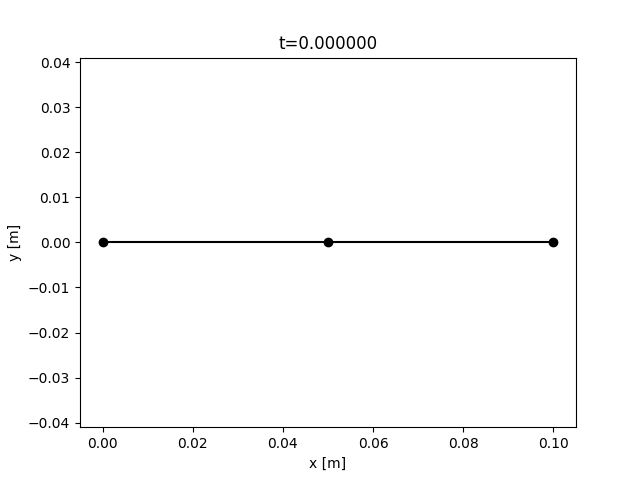
\includegraphics[width=0.45\textwidth,keepaspectratio]{p1q1_implicit_0.00.png}
        \caption{Shape of the structure at t = 0.00}
        \label{"fig:p1q1_0.00"}
\end{figure}

\begin{figure}[!ht]
        \centering
        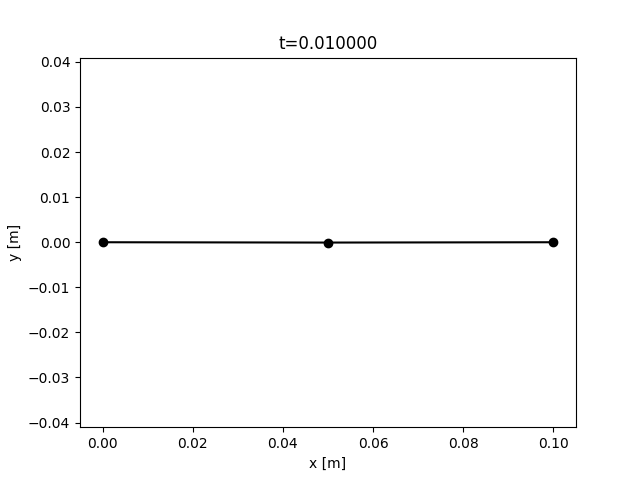
\includegraphics[width=0.45\textwidth,keepaspectratio]{p1q1_implicit_0.01.png}
        \caption{Shape of the structure at t = 0.01}
        \label{"fig:p1q1_0.01"}
\end{figure}


\begin{figure}[!ht]
        \centering
        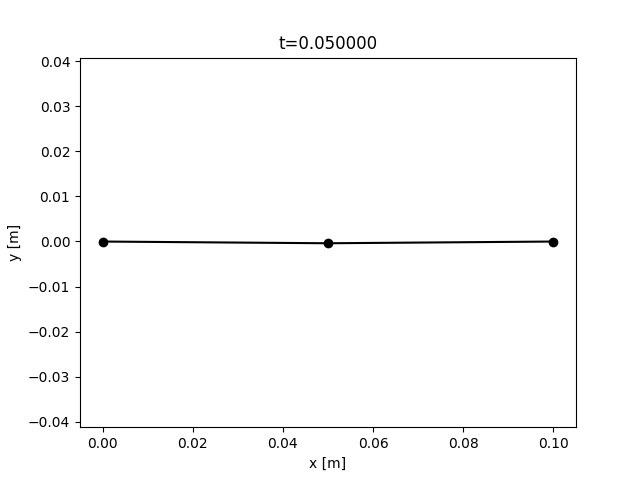
\includegraphics[width=0.45\textwidth,keepaspectratio]{p1q1_implicit_0.05.png}
        \caption{Shape of the structure at t = 0.05}
        \label{"fig:p1q1_0.05"}
\end{figure}


\begin{figure}[!ht]
        \centering
        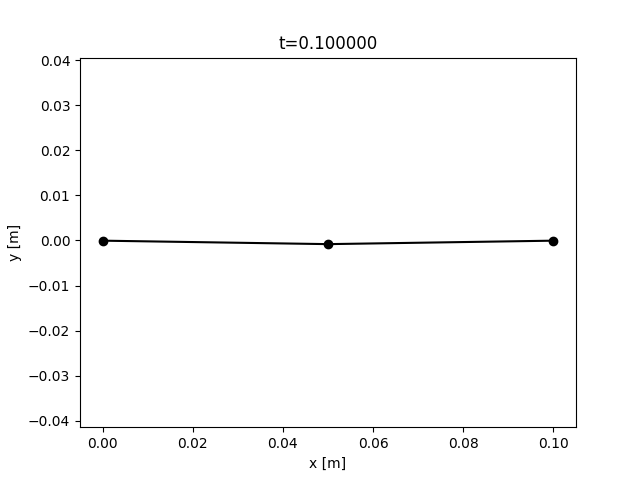
\includegraphics[width=0.45\textwidth,keepaspectratio]{p1q1_implicit_0.10.png}
        \caption{Shape of the structure at t = 0.10}
        \label{"fig:p1q1_0.10"}
\end{figure}


\begin{figure}[!ht]
        \centering
        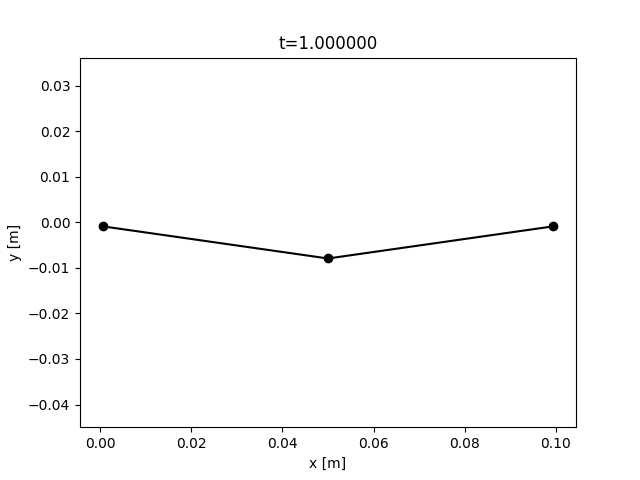
\includegraphics[width=0.45\textwidth,keepaspectratio]{p1q1_implicit_1.00.png}
        \caption{Shape of the structure at t = 1.00}
        \label{"fig:p1q1_1.00"}
\end{figure}


\begin{figure}[!ht]
        \centering
        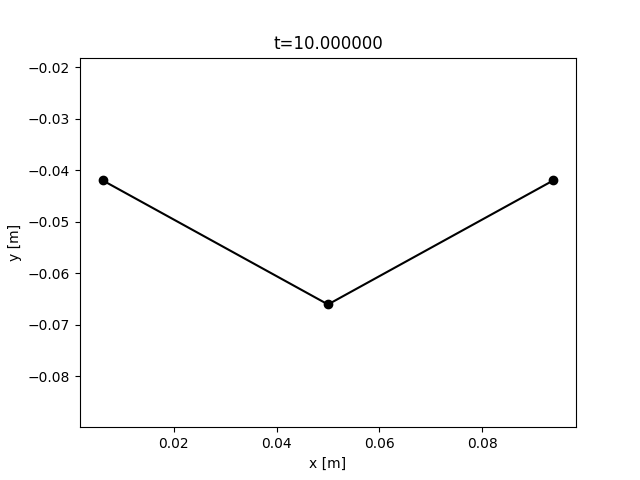
\includegraphics[width=0.45\textwidth,keepaspectratio]{p1q1_implicit_10.00.png}
        \caption{Shape of the structure at t = 10.00}
        \label{"fig:p1q1_10.00"}
\end{figure}


\subsection*{Q1: Position and Velocity Plot of $R_2$  as a function of time($t$)}

The position and velocity (and turning angle) plots of $R_2$ are displayed in Fig. \ref{"fig:p1q1_position"} to Fig. \ref{"fig:p1q1_angle"}. As figured from the shape of the structure over time, the displacement decreases in a near linear fashion. The velocity also decreases, but approaches a terminal velocity as time goes on. Note that the spike in the velocity in the beginning of the graph is due to the initial velocity being set to 0 and the fact that the velocity is calculated using the difference between the current and previous position.

\begin{figure}[!ht]
        \centering
        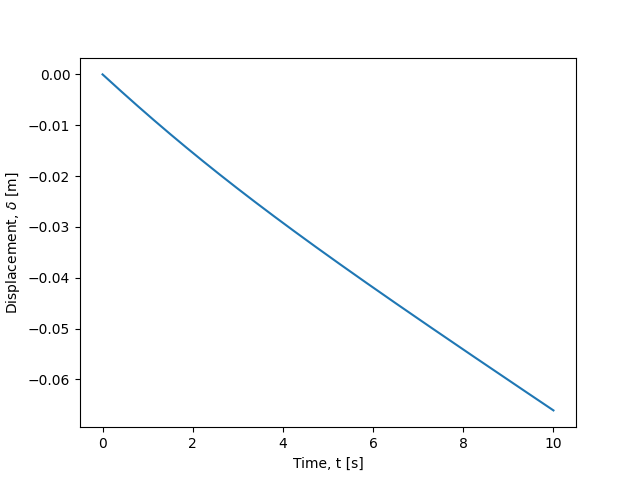
\includegraphics[width=0.45\textwidth,keepaspectratio]{p1q1fallingBeam_p1_implicit.png}
        \caption{Plot of position of $R_2$ v.s. t}
        \label{"fig:p1q1_position"}
\end{figure}

\begin{figure}[!ht]
        \centering
        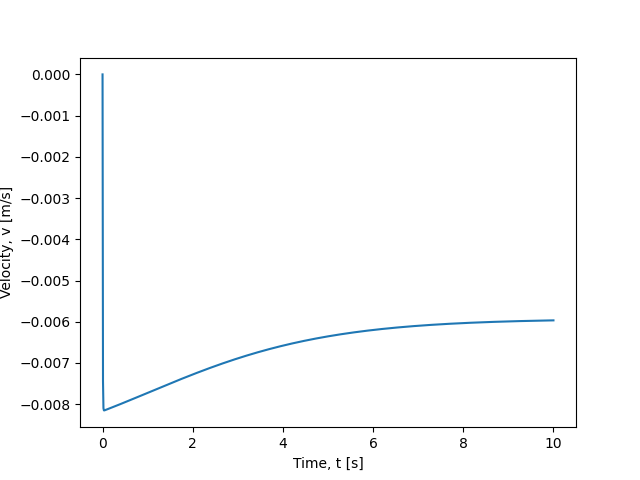
\includegraphics[width=0.45\textwidth,keepaspectratio]{p1q1fallingBeam_velocity_p1_implicit.png}
        \caption{Plot of velocity of $R_2$ v.s. t}
        \label{"fig:p1q1_velocity"}
\end{figure}

\begin{figure}[!ht]
        \centering
        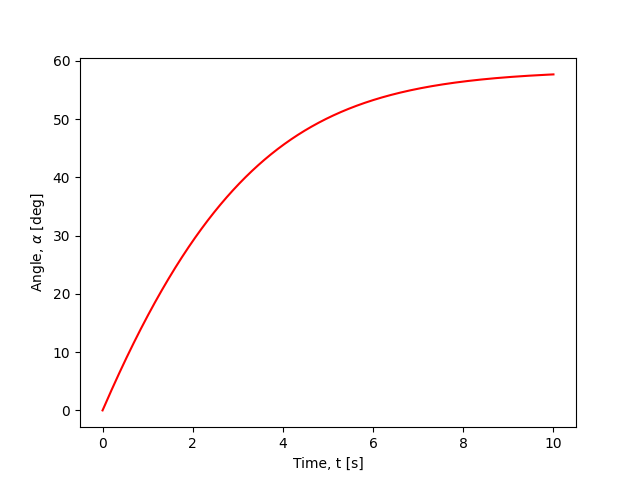
\includegraphics[width=0.45\textwidth,keepaspectratio]{p1q1fallingBeam_angle_p1_implicit.png}
        \caption{Plot of velocity of $R_2$ v.s. t}
        \label{"fig:p1q1_angle"}
\end{figure}


\subsection*{ Q2: Terminal velocity of the system}

The terminal velocity of the system (all 3 spheres) is -0.005926 m/s. We find this by letting the simulation run for a long time (I let the system run until $t=50$, but you could see the convergence starts somewhere between $t=10$ and $t=20$ in Fig. \ref{"fig:p1q2_term_velocity"}) and obtaining the final velocity of the system.

\begin{figure}[!ht]
        \centering
        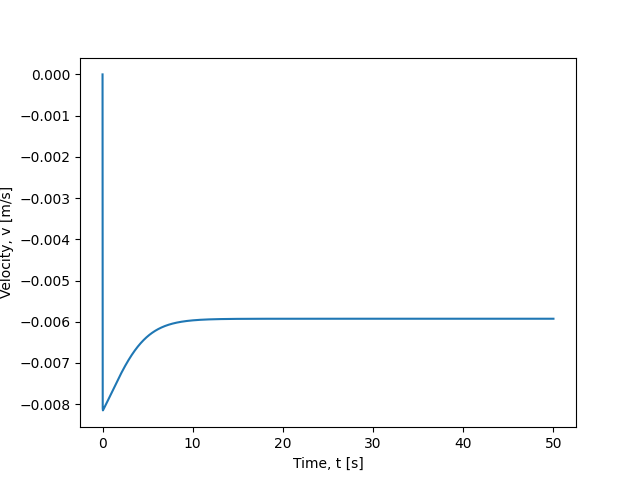
\includegraphics[width=0.45\textwidth,keepaspectratio]{p1q2_implicitfallingBeam_velocity.png}
        \caption{Plot of velocity of $R_2$ v.s. t over 50 seconds}
        \label{"fig:p1q2_term_velocity"}
\end{figure}

\subsection*{ Q3: What happens to the turning angle if all radii are the same? }

If all the radii of the spheres are the same the turning angle will remain 0. Gravity acts on each part of the beam with equal force, so each sphere has the same acceleration and the same velocity. Because they all started at the same y, their displacements will also remain the same. So the turning angle remains what it was in the initial condition, which is 0 degrees. The final shape and turning angle graph is shown in Fig. \ref{"fig:p1q3_turning_angle"} and Fig. \ref{"fig:p1q3_final_shape"}.

\begin{figure}[!ht]
        \centering
        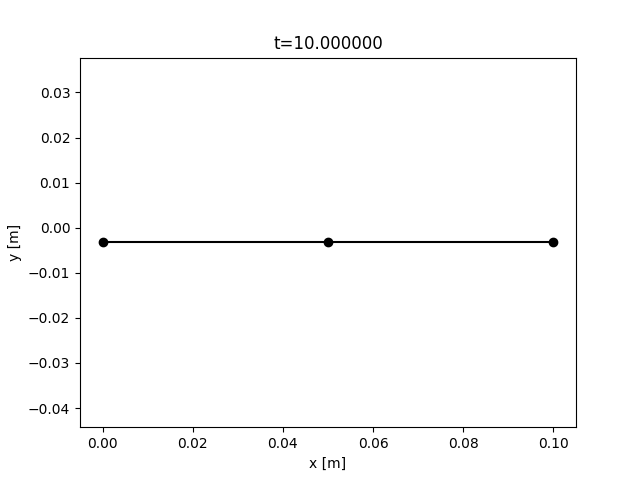
\includegraphics[width=0.45\textwidth,keepaspectratio]{p1q3_implicit_10.00.png}
        \caption{Final shape of the structure with spheres of same radii at t = 10.00}
        \label{"fig:p1q3_final_shape"}
\end{figure}

\begin{figure}[!ht]
        \centering
        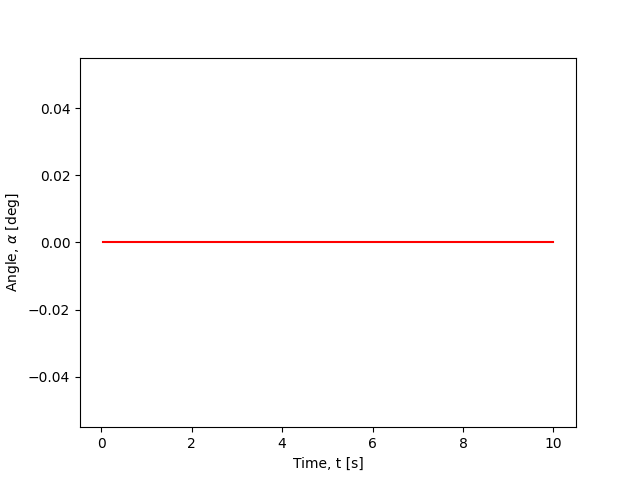
\includegraphics[width=0.45\textwidth,keepaspectratio]{p1q3_implicit_fallingBeam_angle.png}
        \caption{Plot of turning angle at $R_2$ of structure with spheres of same radii}
        \label{"fig:p1q3_turning_angle"}
\end{figure}


\subsection*{ Q4: What happens when we change the time step, specifically for the explicit simulation?}
At larger time steps, the explicit simulation completes faster, but has a harder time converging. As an example, when $\Delta t = 1.0 \times  10^2$, the simulation warns of scalar overflow errors (graph is shown in Figure \ref{"fig:p1q4_bad_graph"}). This behavior emerges from the fact that our simulation relies on discretized formulas to compute an approximation. These discretizations theoretically assume an infinitesimally small time step, which is impossible for a computer to simulate. So we use a finite time step which contributes to an accumulation of error (there is no way to estimate that a value is within the neighborhood of a ground truth, since we aren't using an approximating algorithm like Newton's method). The error eventually causes values to diverge from their analytical truths and spiral out of control. This is why explicit simulations benefit from having small time steps, at the cost of a higher computation time (due to more iterations).

To conclude, one should use an explicit simulation when the computation time is not a concern and accuracy is desired. Otherwise, a implicit simulation should suffice. 

\begin{figure}[!ht]
        \centering
        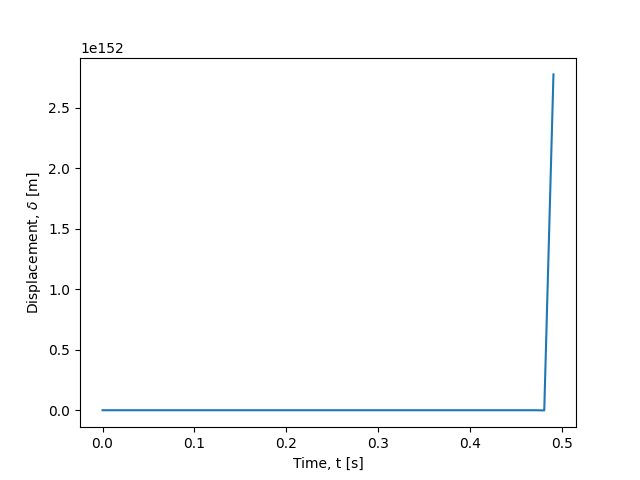
\includegraphics[width=0.45\textwidth,keepaspectratio]{p1q4_explicit_fallingBeam.png}
        \caption{A (bad) plot of the position v.s. time of $R_2$ for explicit simulation. Notice that the graph only goes up to $t=0.5$. This is due to NaN values being generated in the simulation.}
        \label{"fig:p1q4_bad_graph"}
\end{figure}


\section{4.2 Generalized Case of Elastic Beam Falling in Viscous Flow}

In the general case of the elastic beam falling, we have $N = 21$ spheres. We use the same variables as in the previous case, but some variables are calculated differently ( $R = \Delta l / 10$, $\Delta l = l / (N - 1)$ ). The elastic energy is now given by the following equation:

\begin{center}
        $E^{\text{Elastic}} = \sum\limits_{j=1}^{N-1} E^S_j + \sum\limits_{j=1}^{N-1} E^b_j $
\end{center}

and the Jacobian matrix is given by the following equation:

\begin{center}

        $ \mathbb{J}_{ij} = \frac{\partial f_i}{ \partial q_j} = \frac{m_i}{\Delta t^2} + \frac{(6 \pi \mu R_i)}{\Delta t} + \frac{\partial^2 E^{\text{Elastic}}}{\partial q_i \partial q_j }$ 
        $\text{where}$ \\

        $\frac{\partial^2 E^{\text{Elastic}}}{\partial q_i \partial q_j} = \sum\limits_{k=1}^{N-1} \frac{\partial^2 E^k_s}{\partial q_i \partial q_j} + \frac{\partial^2 E^b}{\partial q_i \partial q_j} \text{  for  } i = 1, \dots, {N-1} \text{  and  } j = 1, \dots, {N-1}$
        
\end{center}

where $E^S_j$ and $E^b_j$ are the stretching and bending energies of the beam at the $j$th node, respectively. The forces are calculated in such a way that each edge only concerns itself with the nodes it is connected to. The equations of motion for the beam remain the same, just generalized for multiple nodes.

\subsection*{Q1: Plot of position and velocity of middle node as a function of time}

The plots are shown in Fig. \ref{"fig:p2q1_position"} to Fig. \ref{"fig:p2q1_angle"}. The structure exhibits similar behavior to the 3-sphere system, given that the position decreases near linearly and the velocity approaches a terminal velocity.

\begin{figure}[!ht]
        \centering
        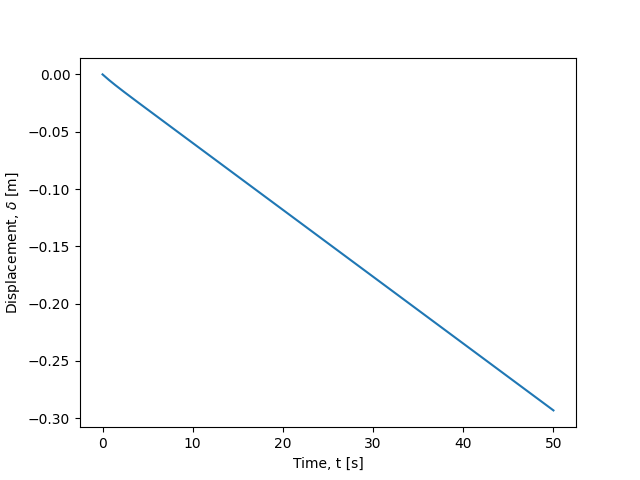
\includegraphics[width=0.45\textwidth,keepaspectratio]{p2q1_implicit_fallingBeam.png}
        \caption{Plot of the position v.s. time of $R_{(N-1)/2}$}
        \label{"fig:p2q1_position"}
\end{figure}

\begin{figure}[!ht]
        \centering
        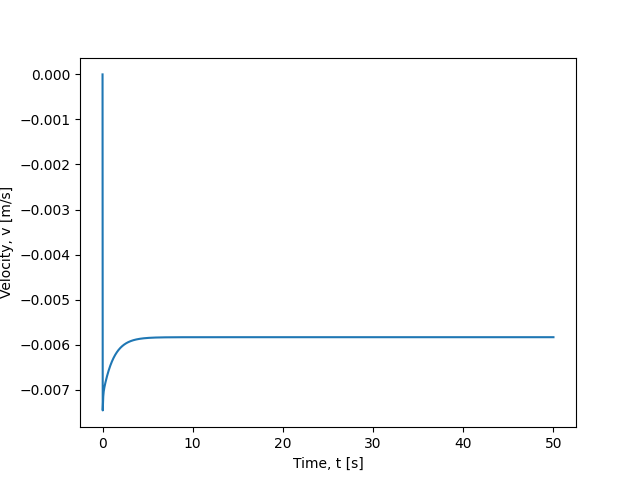
\includegraphics[width=0.45\textwidth,keepaspectratio]{p2q1_implicit_fallingBeam_velocity.png}
        \caption{Plot of the velocity v.s. time of $R_{(N-1)/2}$}
        \label{"fig:p2q1_velocity"}
\end{figure}

\begin{figure}[!ht]
        \centering
        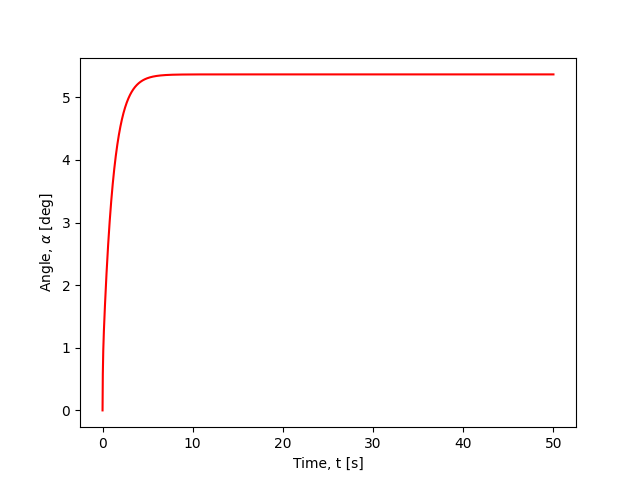
\includegraphics[width=0.45\textwidth,keepaspectratio]{p2q1_implicit_fallingBeam_angle.png}
        \caption{Plot of the turning angle v.s. time of $R_{(N-1)/2}$}
        \label{"fig:p2q1_angle"}
\end{figure}

\subsection*{Q2: Final shape of deformed beam}

The final shape of the beam is shown in Fig. \ref{"fig:p2q2_final_shape"}. The beam is bent in a similar fashion to the 3-sphere system, but the bend is more pronounced because there are more nodes (it looks like a hanging rope).

\begin{figure}[!ht]
        \centering
        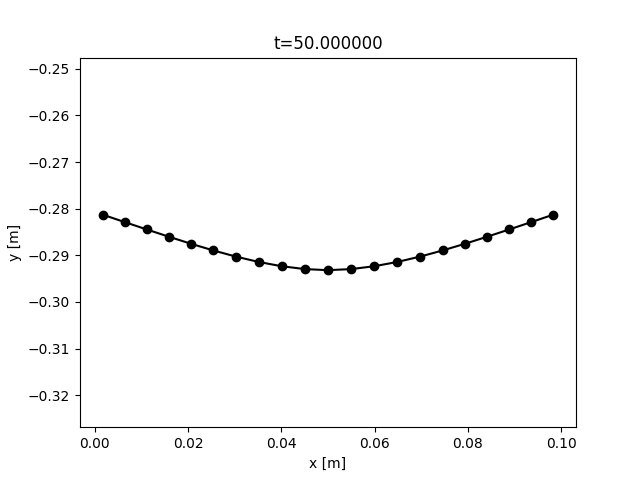
\includegraphics[width=0.45\textwidth,keepaspectratio]{p2q2_implicit_50.00.png}
        \caption{Final shape of the structure at t = 50.00}
        \label{"fig:p2q2_final_shape"}
\end{figure}

\subsection*{Q3: What is the significance of spatial discretization (N nodes) and temporal discretization($\Delta t$)? }

Increasing (as in creating more tinier subdivisions) spatial discretization and temporal discretization leads to more accurate simulations. For spatial discretization In Fig. \ref{"fig:p2q3_spatial"}, we see that the terminal velocity of the system converges as the number of nodes increases. This happens because as the number of nodes increases, the granularity of our simulation increases, leading to a more precision. In other words, the system is more akin to the continuous system we are trying to simulate. This logic also applies to temporal discretization. In Fig. \ref{"fig:p2q3_temporal"}, we see that the terminal velocity of the system converges as the time step size decreases. The reason this happens is also the same as before, more granularity leads to more precision. So to tune a simulation for a model, one should try increasing the number of nodes and decreasing the time step size until they reach a balance between accuracy and computation time.

\begin{figure}[!ht]
        \centering
        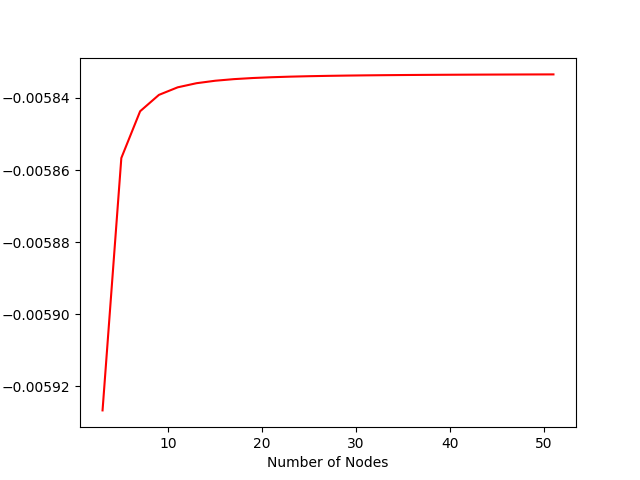
\includegraphics[width=0.45\textwidth,keepaspectratio]{p2q3_implicit_vterm_vs_nodes.png}
        \caption{A plot of the terminal velocity of the system v.s. the number of nodes.}
        \label{"fig:p2q3_spatial"}
\end{figure}

\begin{figure}[!ht]
        \centering
        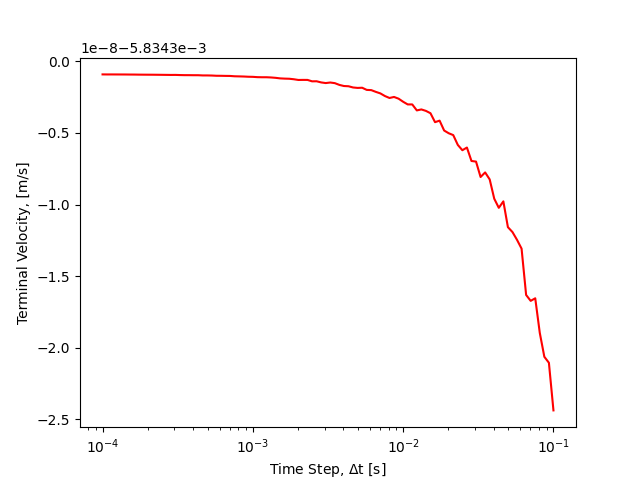
\includegraphics[width=0.45\textwidth,keepaspectratio]{p2q3_implicit_vterm_vs_dt.png}
        \caption{A (logarithmic) plot of the terminal velocity of the system v.s. the time step size.}
        \label{"fig:p2q3_temporal"}
\end{figure}


\section{4.3 Elastic Beam Bending}

\subsection*{Q1: Plot maximum vertical displacement of beam as a function of time. Compare it with the theoretical prediction from the Euler beam theory.}

The plot is shown in Fig. \ref{"fig:p3q1_max_vert"}. We see that the graph of  $y_{\text{max}}$ is steady, suggesting that it converges. The theoretical prediction from the Euler beam theory for $P = 2000$ is given by $y_{\text{max}} = \frac{Pc(L^2-c^2)^1.5}{9\sqrt{3} E I l}$. Using that formula yields $y_{\text{theo} = -0.03804491}$, compared to $y_\text{sim}=0.03710928$. The simulation is off by 0.001, which is a small error. This error is likely due to the fact that the Euler beam theory is as various assumptions that can be relaxed in our simulation (i.e. our simulation supports large deflections, while the Euler beam theory does not). Fig. \ref{"fig:p3q1_beam2000"} shows the beams final configuration.

\begin{figure}[!ht]
        \centering
        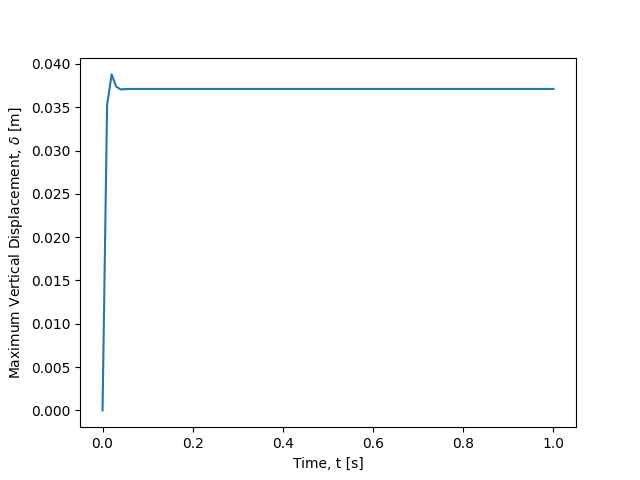
\includegraphics[width=0.45\textwidth,keepaspectratio]{p3q1_implicit_fallingBeam.png}
        \caption{Plot of Maximum Vertical Displacement of the Beam v.s. time}
        \label{"fig:p3q1_max_vert"}
\end{figure}

\begin{figure}[!ht]
        \centering
        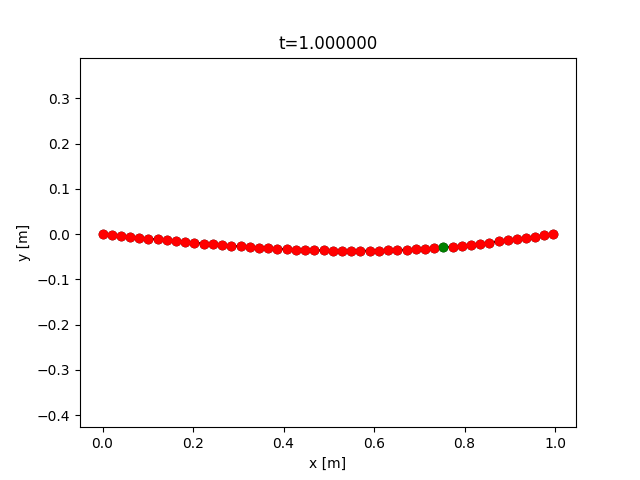
\includegraphics[width=0.45\textwidth,keepaspectratio]{p3q1_implicit_2000.png}
        \caption{Final Shape of the Beam for P = 2000}
        \label{"fig:p3q1_beam2000"}
\end{figure}

\subsection*{Q2: What is the benefit of the simulation over the predictions of the Euler Beam Theory?}

Comparing our results for $P = 20000$, the Euler Beam Theory predicts $y_{\text{theo}} = -0.38044915$, while our simulation predicts $y_{\text{sim}} = -0.23525626$. The error is now 0.15, which is much larger than the error for $P = 2000$. This is because the Euler Beam Theory is only accurate for small deflections and our point load is too large.

In fact, Fig. \ref{"fig:p3q2_benefit"} plots a graph of the maximum vertical displacement of the beam v.s. the size of the point load. We see that the simulation finds the maximum vertical displacement grow nonlinearly while the Euler Beam Theory predicts a linear growth. If we zoom in specifically at the region where $P \leq 5000$ (Fig. \ref{"fig:p3q2_benefit_zoomed"}), we find that the maximum vertical displacement varies by less than 0.01. Zooming even further to $P \leq 100$ (Fig. \ref{"fig:p3q2_benefit_zoomed2x"}), we see that the error is less than 0.001, which confirms the authenticity of our simulation. To pinpoint where the 2 solutions diverges would be difficult because it seems the predictions has always been slightly divergent from one another (by small degrees of significance). But we could say that it is definitely a load less than 5000 N from our first image. 

Fig. \ref{"fig:p3q1_beam20000"} shows the final configuration of the beam for $P = 20000$.

\begin{figure}[!ht]
        \centering
        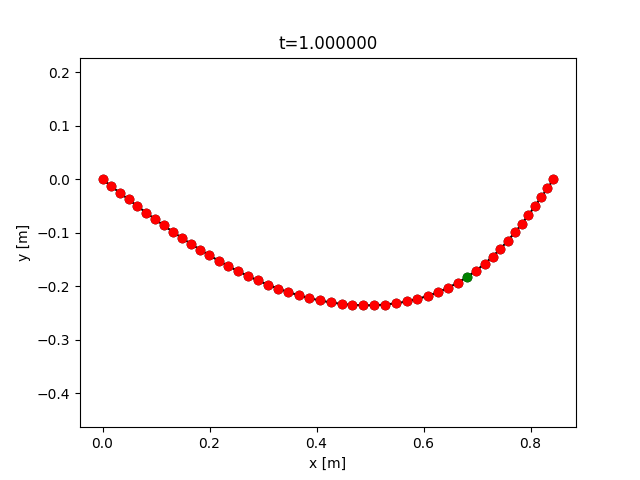
\includegraphics[width=0.45\textwidth,keepaspectratio]{p3q2_implicit_20000.png}
        \caption{Final Shape of the Beam for P = 20000}
        \label{"fig:p3q1_beam20000"}
\end{figure}


\begin{figure}[!ht]
        \centering
        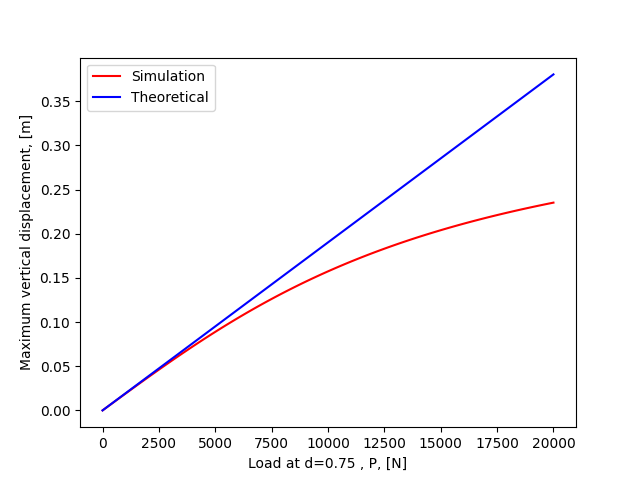
\includegraphics[width=0.45\textwidth,keepaspectratio]{p3q2_implicit_maxvert.png}
        \caption{Plot of Maximum Vertical Displacement of the Beam v.s. the size of the point load}
        \label{"fig:p3q2_benefit"}
\end{figure}


\begin{figure}[!ht]
        \centering
        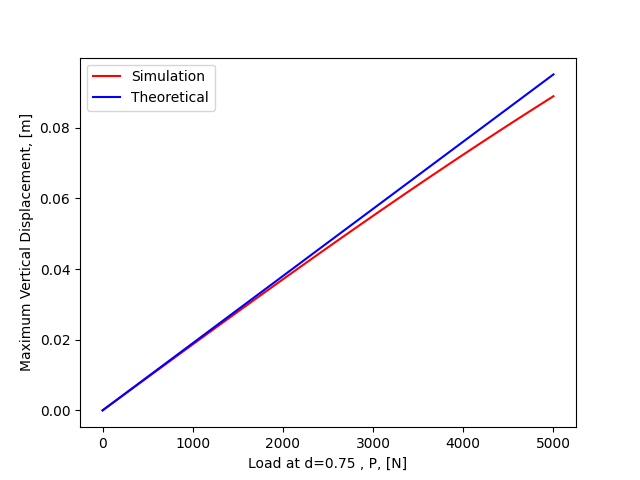
\includegraphics[width=0.45\textwidth,keepaspectratio]{p3q2_implicit_maxvert_zoomed.png}
        \caption{Plot of Maximum Vertical Displacement of the Beam v.s. the size of the point load (zoomed in)}
        \label{"fig:p3q2_benefit_zoomed"}
\end{figure}

\begin{figure}[!ht]
        \centering
        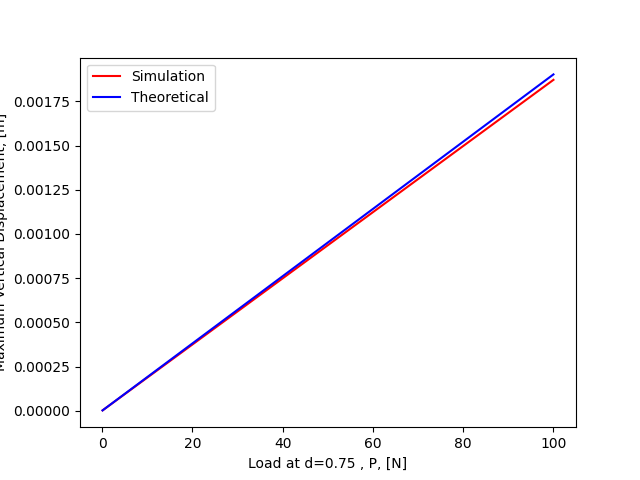
\includegraphics[width=0.45\textwidth,keepaspectratio]{p3_implicit_maxvert2xzoomed.png}
        \caption{Plot of Maximum Vertical Displacement of the Beam v.s. the size of the point load (zoomed in again)}
        \label{"fig:p3q2_benefit_zoomed2x"}
\end{figure}

\addtolength{\textheight}{-12cm}   % This command serves to balance the column lengths
                                  % on the last page of the document manually. It shortens
                                  % the textheight of the last page by a suitable amount.
                                  % This command does not take effect until the next page
                                  % so it should come on the page before the last. Make
                                  % sure that you do not shorten the textheight too much.

%%%%%%%%%%%%%%%%%%%%%%%%%%%%%%%%%%%%%%%%%%%%%%%%%%%%%%%%%%%%%%%%%%%%%%%%%%%%%%%%



%%%%%%%%%%%%%%%%%%%%%%%%%%%%%%%%%%%%%%%%%%%%%%%%%%%%%%%%%%%%%%%%%%%%%%%%%%%%%%%%



\end{document}
